% Created 2021-07-02 Fri 21:43
% Intended LaTeX compiler: pdflatex
\documentclass[11pt]{article}
\usepackage[utf8]{inputenc}
\usepackage[T1]{fontenc}
\usepackage{graphicx}
\usepackage{grffile}
\usepackage{longtable}
\usepackage{wrapfig}
\usepackage{rotating}
\usepackage[normalem]{ulem}
\usepackage{amsmath}
\usepackage{textcomp}
\usepackage{amssymb}
\usepackage{capt-of}
\usepackage{hyperref}
\graphicspath{{../../books/}}
% TIPS
% \substack{a\\b} for multiple lines text





% pdfplots will load xolor automatically without option
\usepackage[dvipsnames]{xcolor}

\usepackage{forest}
% two-line text in node by [two \\ lines]
% \begin{forest} qtree, [..] \end{forest}
\forestset{
  qtree/.style={
    baseline,
    for tree={
      parent anchor=south,
      child anchor=north,
      align=center,
      inner sep=1pt,
    }}}
%\usepackage{flexisym}
% load order of mathtools and mathabx, otherwise conflict overbrace

\usepackage{mathtools}
%\usepackage{fourier}
\usepackage{pgfplots}
\usepackage{amsthm, mathabx,  amsmath, commath}
\usepackage{amsfonts}

\usepackage{empheq}
\usepackage{tikz}
\usetikzlibrary{arrows.meta}
\usepackage[most]{tcolorbox}

\newtheorem{theorem}{Theorem}[section]
\newtheorem{definition}{Definition}[section]
\newtheorem{corollary}{Corollary}[section]
\newtheorem{example}{Example}[section]
\newtheorem{lemma}{Lemma}[section]
\newtheorem{proposition}{Proposition}[section]

\newcommand{\bl}[1] {\boldsymbol{#1}}
\newcommand{\Wt}[1] {\stackrel{\sim}{\smash{#1}\rule{0pt}{1.1ex}}}
\newcommand{\wt}[1] {\widetilde{#1}}


%For boxed texts in align, use Aboxed{}
%otherwise use boxed{}

\DeclareMathSymbol{\widehatsym}{\mathord}{largesymbols}{"62}
\newcommand\lowerwidehatsym{%
  \text{\smash{\raisebox{-1.3ex}{%
    $\widehatsym$}}}}
\newcommand\fixwidehat[1]{%
  \mathchoice
    {\accentset{\displaystyle\lowerwidehatsym}{#1}}
    {\accentset{\textstyle\lowerwidehatsym}{#1}}
    {\accentset{\scriptstyle\lowerwidehatsym}{#1}}
    {\accentset{\scriptscriptstyle\lowerwidehatsym}{#1}}
}

\usepackage{graphicx}
    
% text on arrow for xRightarrow
\makeatletter
%\newcommand{\xRightarrow}[2][]{\ext@arrow 0359\Rightarrowfill@{#1}{#2}}
\makeatother


\def \bx {\boldsymbol{x}}
\def \ba {\boldsymbol{a}}
\def \bI {\boldsymbol{I}}
\def \bt {\boldsymbol{t}}
\def \bb {\boldsymbol{b}}
\def \bA {\boldsymbol{A}}
\def \bX {\boldsymbol{X}}
\def \bu {\boldsymbol{u}}
\def \bS {\boldsymbol{S}}
\def \bZ {\boldsymbol{Z}}
\def \bz {\boldsymbol{z}}
\def \by {\boldsymbol{y}}
\def \bw {\boldsymbol{w}}
\def \bT {\boldsymbol{T}}
\def \bS {\boldsymbol{S}}
\def \bm {\boldsymbol{m}}
\def \bW {\boldsymbol{W}}
\def \bY {\boldsymbol{Y}}
\def \bH {\boldsymbol{H}}
\def \blambda {\boldsymbol{\lambda}}
\def \bPhi {\boldsymbol{\Phi}}
\def \btheta {\boldsymbol{\theta}}
\def \bmu {\boldsymbol{\mu}}
\def \bphi {\boldsymbol{\phi}}
\def \bSigma {\boldsymbol{\Sigma}}
\def \lb {\left\{}
\def \rb {\right\}}
\def \caln {\mathcal{N}}
\def \dissum {\displaystyle\Sigma}
\def \dispro {\displaystyle\prod}
\def \E {\mathbb{E}}
\def \Q {\mathbb{Q}}
\def \V {\mathbb{V}}
\def \R {\mathbb{R}}
\def \calq {\mathcal{Q}}
\def \calg {\mathcal{G}}
\def \caln {\mathcal{N}}
\def \calr {\mathcal{R}}
\def \calm {\mathcal{M}}
\def \calc {\mathcal{C}}
\def \bcup {\bigcup}

\makeindex
\author{Rotman}
\date{\today}
\title{An Introduction To Algebraic Topology}
\hypersetup{
 pdfauthor={Rotman},
 pdftitle={An Introduction To Algebraic Topology},
 pdfkeywords={},
 pdfsubject={},
 pdfcreator={Emacs 27.2 (Org mode 9.5)}, 
 pdflang={English}}
\begin{document}

\maketitle
\tableofcontents


\section{Introduction}
\label{sec:org932f318}

\subsection{Notation}
\label{sec:org986f4a0}
\(\bI=[0,1]\).
\begin{equation*}
S^n=\{x\in\R^{n+1}\mid\norm{x}=1\}
\end{equation*}
\(S^n\) is called the \textbf{\(n\)-sphere}. \(S^n\subset\R^{n+1}\) (\(S^1\) is the circle); 0-sphere \(S^0\)
consists of the two points \(\{-1,1\}\) and hence is a discrete two-point space. We may
regard \(S^n\) as the \textbf{equator} of \(S^{n+1}\)
\begin{equation*}
S^n=\R^{n+1}\cap S^{n+1}=\{(x_1,\dots,x_{n+2})\in S^{n+1}:x_{n+2}=0\}
\end{equation*}
The \textbf{north pole} is \((0,0,\dots,0,1)\in S^n\); the \textbf{south pole} is \((0,0,\dots,0,-1)\). The \textbf{antipode}
of \(x=(x_1,\dots,x_{n+1})\in S^n\) is the other endpoint of the diameter having one endpoint \(x\); thus
the antipode of \(x\) is \(-x=(-x_1,\dots,-x_{n+1})\), for the distance from \(-x\) to \(x\) is 2.
\begin{equation*}
D^n=\{x\in\R^n\mid\norm{x}\le 1\}
\end{equation*}
\(D^n\) is called the \textbf{\(n\)-disk} (or \textbf{\(n\)-ball}).  Observe that \(S^{n-1}\subset D^n\subset \R^n\);
indeed \(S^{n-1}\) is the boundary of \(D^n\) in \(\R^n\)
\begin{equation*}
\Delta^n=\{(x_1,\dots,x_{n+1})\in\R^{n+1}:\text{ each }x_i\ge 0\text{ and }\sum x_i=1\}
\end{equation*}
\(\Delta^n\) is called the \textbf{standard \(n\)-simplex}. \(\Delta^0\) is a point, \(\Delta^1\) is a closed
interval, \(\Delta^2\) is a triangle (with interior), \(\Delta^3\) is a (solid) tetrahedron, and so on.

There is a standard homeomorphism from \(S^n\) - \{north pole\} to \(\R^n\), called \textbf{stereographic
projection}. Denote the north pole by \(N\), and define \(\sigma:S^n-\{N\}\to\R^n\) to be the intersection
of \(\R^n\) and the line joining \(x\) and \(N\). Points on the latter line have the
form \(tx+(1-t)N\), hence they have coordinates
\((tx_1,\dots,tx_n,tx_{n+1}+(1-t))\). The last coordinate is zero for \(t=(1-x_{n+1})^{-1}\); hence
\begin{equation*}
\sigma(x)=(tx_1,\dots,tx_n)
\end{equation*}
where \(t=(1-x_{n+1})^{-1}\). It is now routine to check that \(\sigma\) is indeed a homeomorphism. Note
that \(\sigma(x)=x\) iff \(x\) lies on the equator \(S^{n-1}\)

\subsection{Brouwer Fixed Point Theorem}
\label{sec:orgd27fa8f}
\begin{theorem}[]
Every continuous \(f:D^1\to D^1\) has a fixed point
\end{theorem}

\begin{proof}
Let \(f(-1)=a\) and \(f(1)=b\).If either \(f(-1)=-1\) or \(f(1)=1\), we are done. Therefore we
may assume that \(f(-1)=a>-1\) and that \(f(1)=b<1\) as drawn.
\begin{figure}[htbp]
\centering
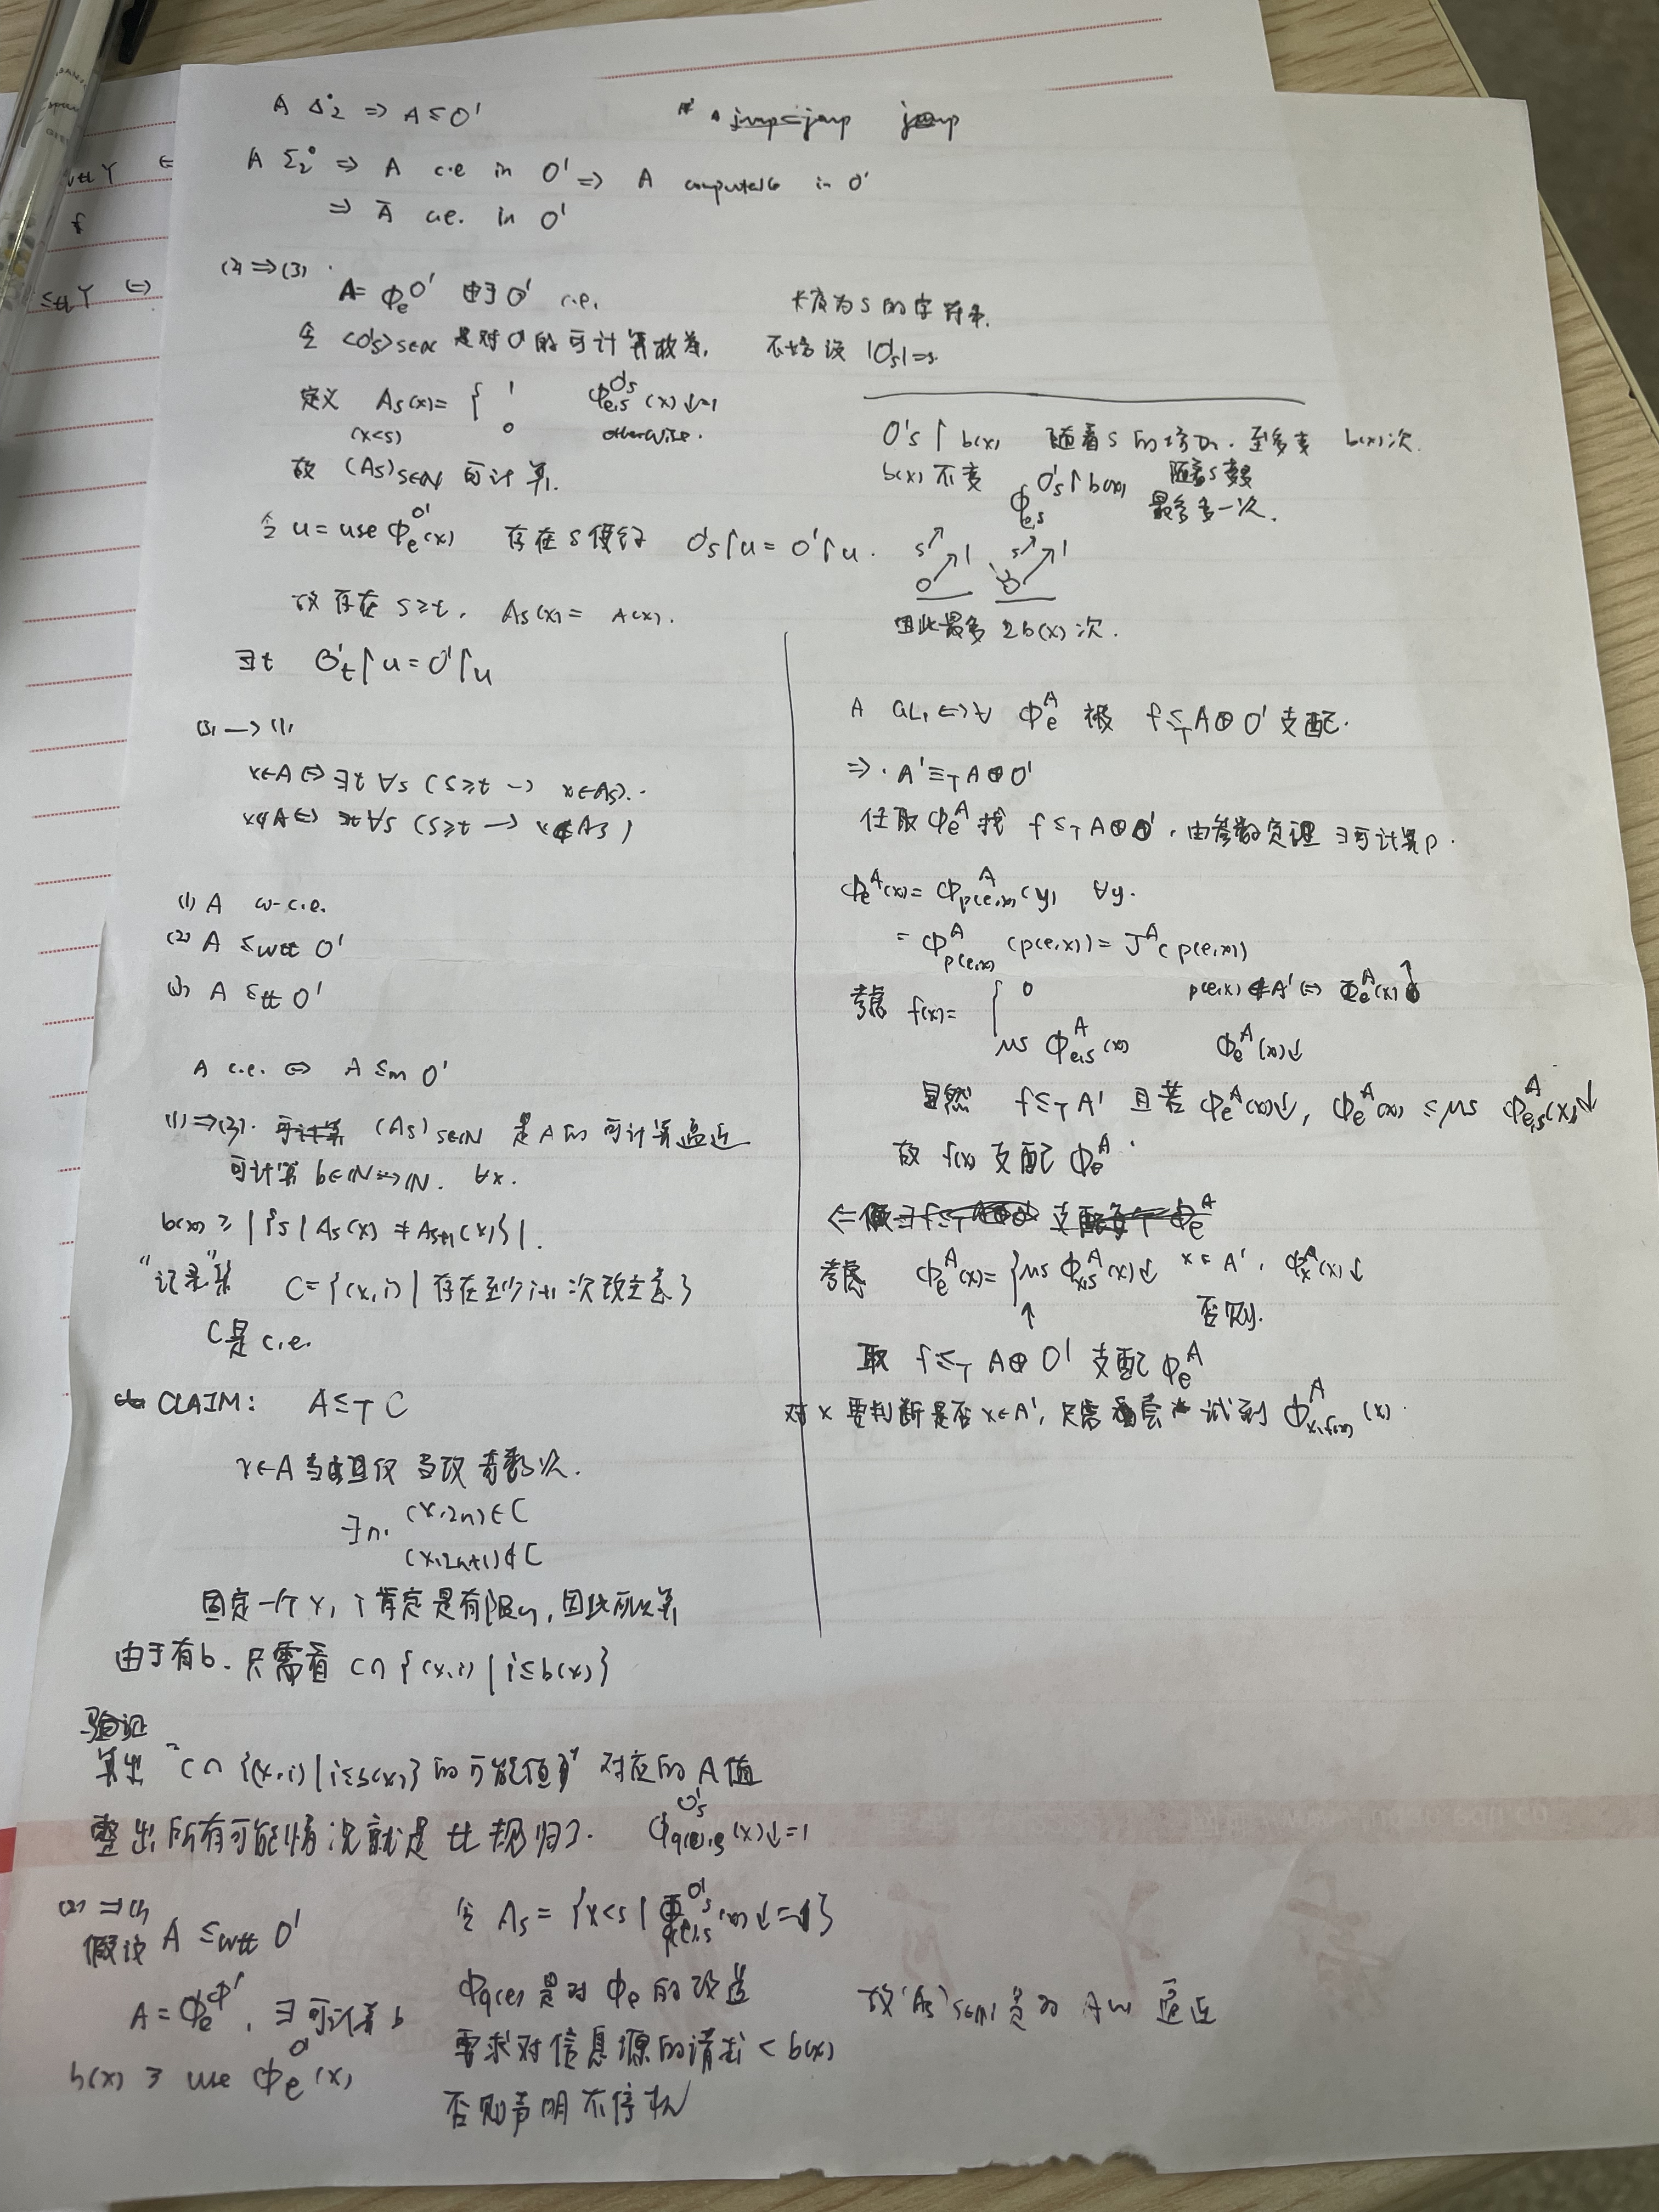
\includegraphics[width=.5\textwidth]{../images/AnIntroductionToAlgebraicTopology/1.png}
\label{}
\end{figure}
If \(G\) is the graph of \(f\) and \(\Delta\) is the graph of the identity function, then we must prove
that \(G\cap\Delta\neq\emptyset\). The idea is to use a connectness argument to show that every path in \(D^1\times D^1\)
from \(a\) to \(b\) must cross \(\Delta\).

Since \(f\) is continuous, \(G=\{(x,f(x)):x\in D^1\}\) is connected (continuous image of connected
space is connected). Define \(A=\{(x,f(x)):f(x)>x\}\)  and \(B=\{(x,f(x)):f(x)<x\}\). Note
that \(a\in A\) and \(b\in B\), so that \(A\neq\emptyset\) and \(B\neq\emptyset\). If \(G\cap\Delta=\emptyset\), then \(G\) is the disjoint
union of \(A\) and \(B\).
\end{proof}


\begin{theorem}[Brouwer fixed point theorem]
If \(f:D^n\to D^n\) is continuous, then there exists \(x\in D^n\) with \(f(x)=x\)
\end{theorem}

\subsection{Categories and Functors}
\label{sec:orgd1bedcb}
\begin{definition}[]
A category \(\calc\) consists of three ingredients: a class of \textbf{objects}, \(\obj\calc\); sets of
\textbf{morphisms} \(\Hom(A,B)\), one for every ordered pair \(A,B\in\obj\calc\);
\textbf{composition} \(\Hom(A,B)\times\Hom(B,C)\to\Hom(A,C)\), denoted by \((f,g)\to g\circ f\), for
every \(A,B,C\in\obj\calc\) satisfying the following axioms
\begin{enumerate}
\item the family of \(\Hom(A,B)\)'s is pairwise disjoint'
\item composition is associative when defined
\item for each \(A\in\obj\calc\) there exists an identity \(1_A\in\Hom(A,A)\) satisfying \(1_A\circ f=f\) for
every \(f\in\Hom(B,A)\), all \(B\in\obj\calc\) and \(g\circ 1_A=g\) for every \(g\in\Hom(A,C)\), all \(C\in\obj\calc\)
\end{enumerate}
\end{definition}

\begin{definition}[]
Let \(\calc\) and \(\cala\) be categories with \(\obj\calc\subset\obj\cala\). If \(A,B\in\obj\calc\), let's denote the two
possible Hom sets by \(\Hom_{\calc}(A,B)\) and \(\Hom_{\cala}(A,B)\). Then \(\calc\) is a \textbf{subcategory}
of \(\cala\) if \(\Hom_{\calc}(A,B)\subset\Hom_{\cala}(A,B)\) for all \(A,B\in\obj\calc\) and if composition in \(\calc\) is
the same as composition in \(\cala\)
\end{definition}

\begin{examplle}[]
\(\calc=\Top^{2}\). here \(\obj\calc\) consists of all ordered pairs \((X,A)\) where \(X\) is a topological
space and \(A\) is a subspace of \(X\). A morphism \(f:(X,A)\to(Y,B)\) is an ordered
pair \((f,f')\) where \(f:X\to Y\) is continuous and \(fi=jf'\) (where \(i\) and \(j\) are
inclusions)
\begin{center}
\begin{tikzcd}
A\arrow[r,hookrightarrow,"i"]\arrow[d,"f'"']&X\arrow[d,"f"]\\
B\arrow[r,hookrightarrow,"j"']&Y
\end{tikzcd}
\end{center}
\end{examplle}




\section{Index}
\label{sec:org0338f5c}
\renewcommand{\indexname}{}
\printindex
\end{document}
